\documentclass{../exhibit}

\title{Tangram Sea}

%% Font
\usepackage{imfellEnglish}
\usepackage[T1]{fontenc}
\raggedright

\usepackage{background}

\backgroundsetup{
scale=1,
color=black,
opacity=0.4,
angle=0,
contents={%
  \includegraphics[height=\paperheight]{mapBackground.jpg}%%https://upload.wikimedia.org/wikipedia/commons/8/81/Nautical_chart_of_the_West_Indies_1797.jpg
  }%
}




%% For the context
%% https://tex.stackexchange.com/questions/86150/torn-page-effect/86151#86151
\usepackage{tikz}
\usetikzlibrary{decorations.pathmorphing}
\definecolor{paper}{RGB}{239,227,157}





\renewcommand{\maketitle}{ %
  \begin{center}
    \scalebox{8}{\thetitle}
  \end{center}
  
\begin{tabular*}{\textwidth}{c @{\extracolsep{\fill}} c}  
\resizebox{4in}{!}{\begin{minipage}[b]{3in}\huge\directions\end{minipage}} &
  \resizebox{4in}{!}{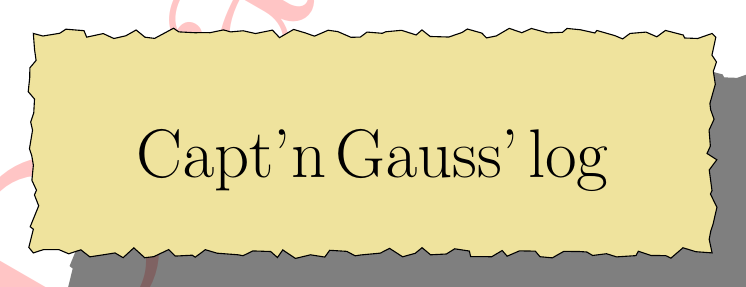
\begin{tikzpicture}[pencildraw/.style={ %
    decorate,
    decoration={random steps,segment length=4pt,amplitude=2pt}
    } %
]
\node[
preaction={fill=black,opacity=.5,transform canvas={xshift=.5cm,yshift=-.5cm}},
pencildraw,draw,fill=paper,text width=3in,inner sep=.5cm] 
{\begin{center}\Huge Capt'n Gauss' log \end{center}\vspace{.7cm} {\huge\context}};
\end{tikzpicture}}

\end{tabular*}

\vfill

\includegraphics[width=3in]{logoPirate.png}\hfill \includegraphics[width=2in]{bammLogo.png}


}


\begin{document}

\begin{context}
  Argg! We be lost in the Tangram Sea!


  Help an old sea dog like me, see through the fog,


  And unlock the secret of


  Tangram Sea!
\end{context}

\begin{directions} To complete a tangram puzzle, you should use all
the pieces to build the desired silouette.  Pieces should be laid flat but they may be rotated or
flipped.  Pieces may not overlap.
\end{directions}

\begin{example}
\begin{tikzpicture}[scale=1]
\pic[tangram] at (0,0) {big triangle};
\pic[tangram,rotate=-90] at (2,2) {big triangle};
\pic[tangram,rotate=-90] at (2,0) {square};
\pic[tangram,rotate=180] at (4,0) {small triangle};
\pic[tangram,rotate=90] at (2,-1) {small triangle};
\pic[tangram,xscale=-1] at (2,-1) {parallelogram};
\pic[tangram,rotate=180] at (3,-1) {medium triangle};
\end{tikzpicture}
\raisebox{1in}{A square is the classic tangram puzzle.}

\hfill \raisebox{0.5in}{But other shapes are possible!}
\begin{tikzpicture}[scale=1]
\path (0,-1) pic[tangram] {small triangle}
++(1,0) pic[tangram] {square}
++(1,1) pic[tangram,rotate=-45,yscale=-1] {big triangle}
++(-45:2) pic[tangram,rotate=-135] {big triangle}
+({-sqrt(2)},0) pic[tangram,rotate=-135] {parallelogram}
++(-2,{-2*sqrt(2)}) pic[tangram] {medium triangle}
++(2,1) pic[tangram,rotate=-90] {small triangle}
;
\end{tikzpicture}

\end{example}



\begin{mathConnections}
  https://bartsnapp.github.io/Math-Outreach-Exhibits/tangrams/
\end{mathConnections}
\end{document}
